\paragraph{Model configuration}

\paragraph{Training}
Objective: Minimize loss function defined as:

\begin{figure}[H]
\centering
\begin{subfigure}[h]{.45\linewidth}
    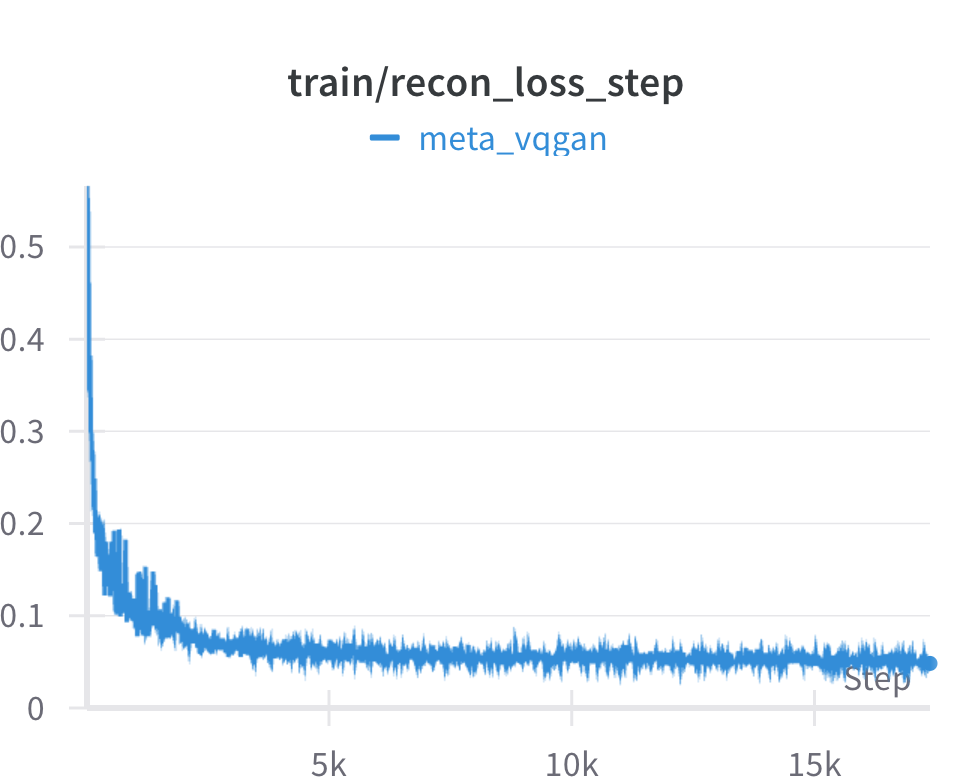
\includegraphics[width=\linewidth]{detailed_engineering/Meta VQGAN/charts/train_recon_loss_step.png}
    \caption{Caption}
    \label{fig:enter-label}
\end{subfigure}
\hfill
\begin{subfigure}[h]{.45\linewidth}
    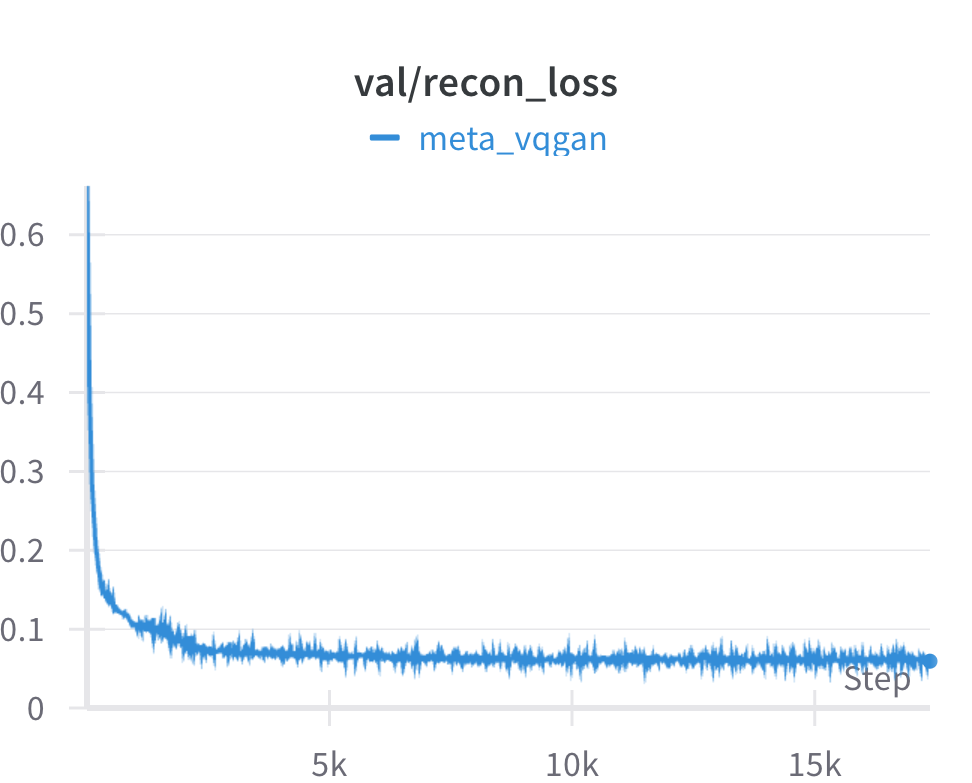
\includegraphics[width=\linewidth]{detailed_engineering/Meta VQGAN/charts/val_recon_loss.png}
    \caption{Caption}
    \label{fig:enter-label}
\end{subfigure}
\hfill
\begin{subfigure}[h]{.45\linewidth}
    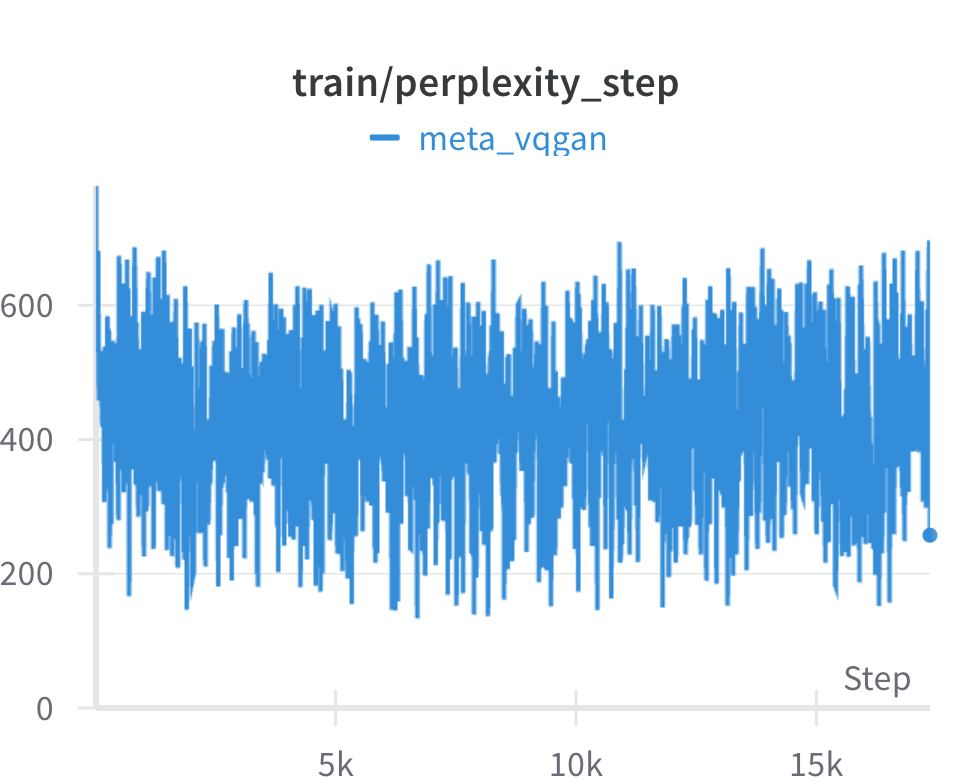
\includegraphics[width=\linewidth]{detailed_engineering/Meta VQGAN/charts/train_perplexity_step.png}
    \caption{Caption}
    \label{fig:enter-label}
\end{subfigure}
\hfill
\begin{subfigure}[h]{.45\linewidth}
    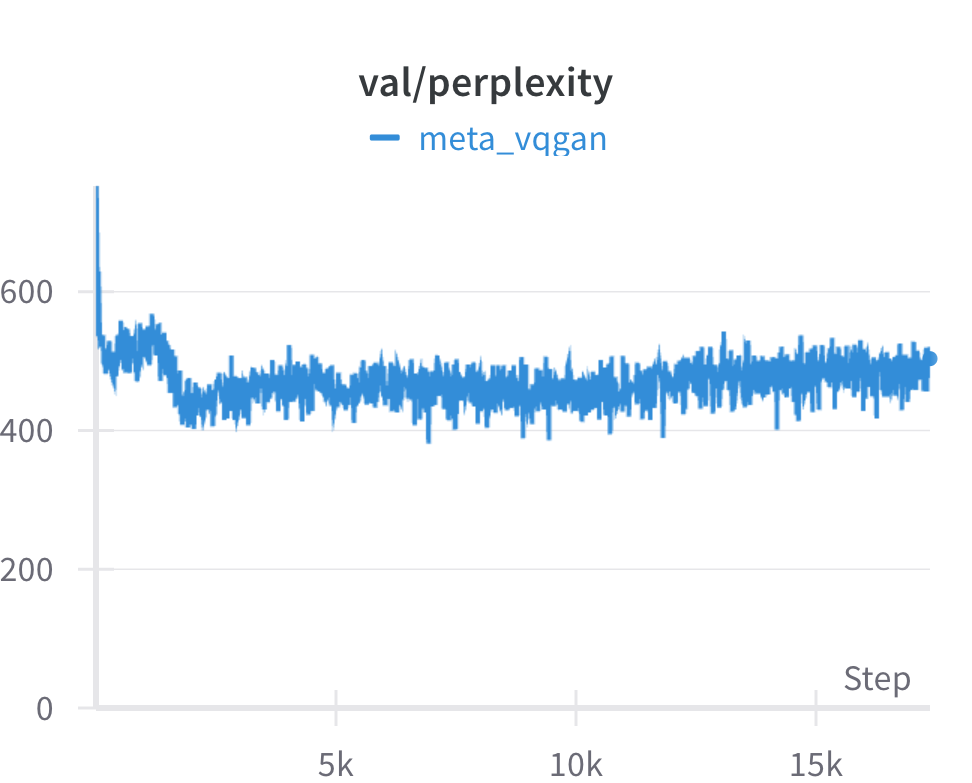
\includegraphics[width=\linewidth]{detailed_engineering/Meta VQGAN/charts/val_perplexity.png}
    \caption{Caption}
    \label{fig:enter-label}
\end{subfigure}
\hfill
\begin{subfigure}[h]{.45\linewidth}
    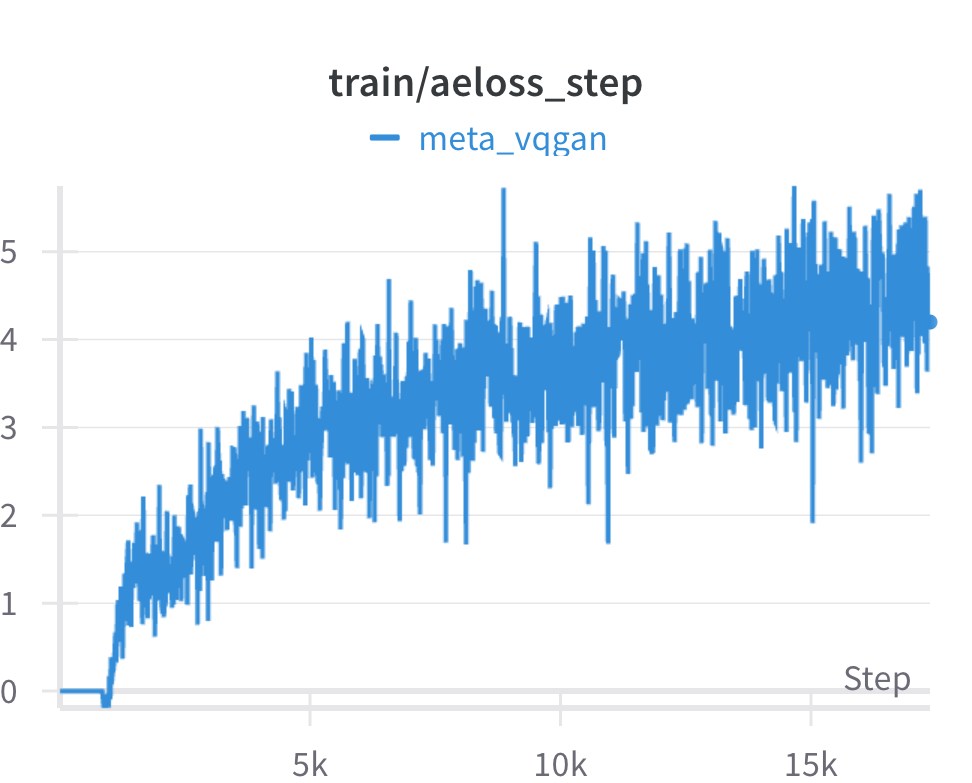
\includegraphics[width=\linewidth]{detailed_engineering/Meta VQGAN/charts/train_aeloss_step.png}
    \caption{Caption}
    \label{fig:enter-label}
\end{subfigure}
\hfill
\begin{subfigure}[h]{.45\linewidth}
    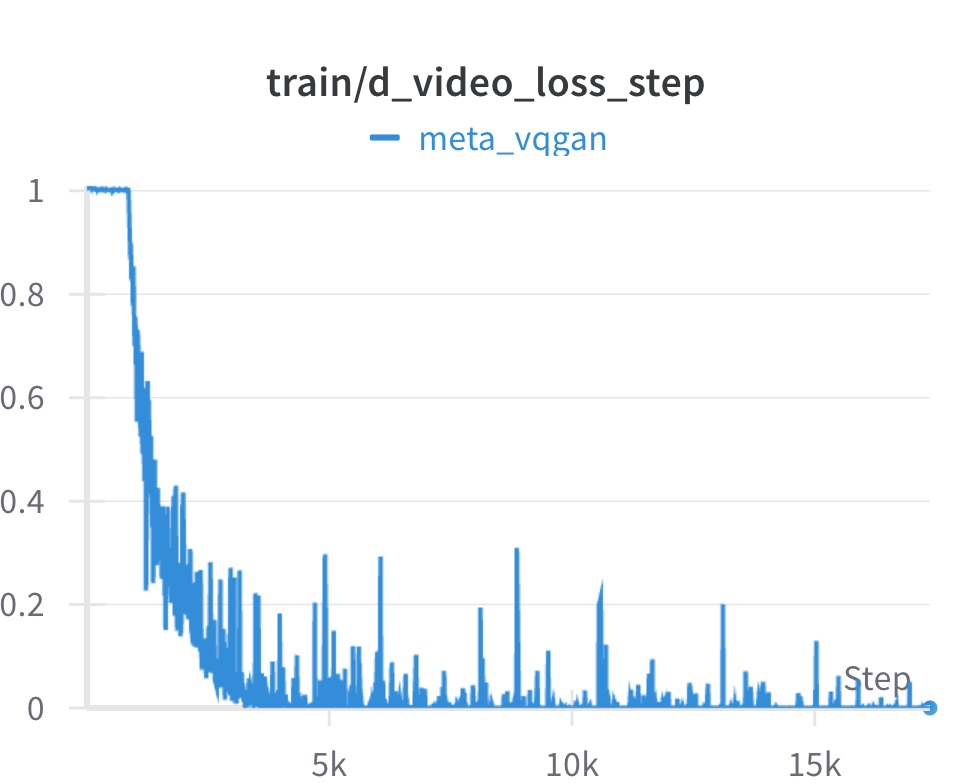
\includegraphics[width=\linewidth]{detailed_engineering/Meta VQGAN/charts/train_d_video_loss_step.png}
    \caption{Caption}
    \label{fig:enter-label}
\end{subfigure}
\hfill
% \begin{subfigure}[h]{.45\linewidth}
%     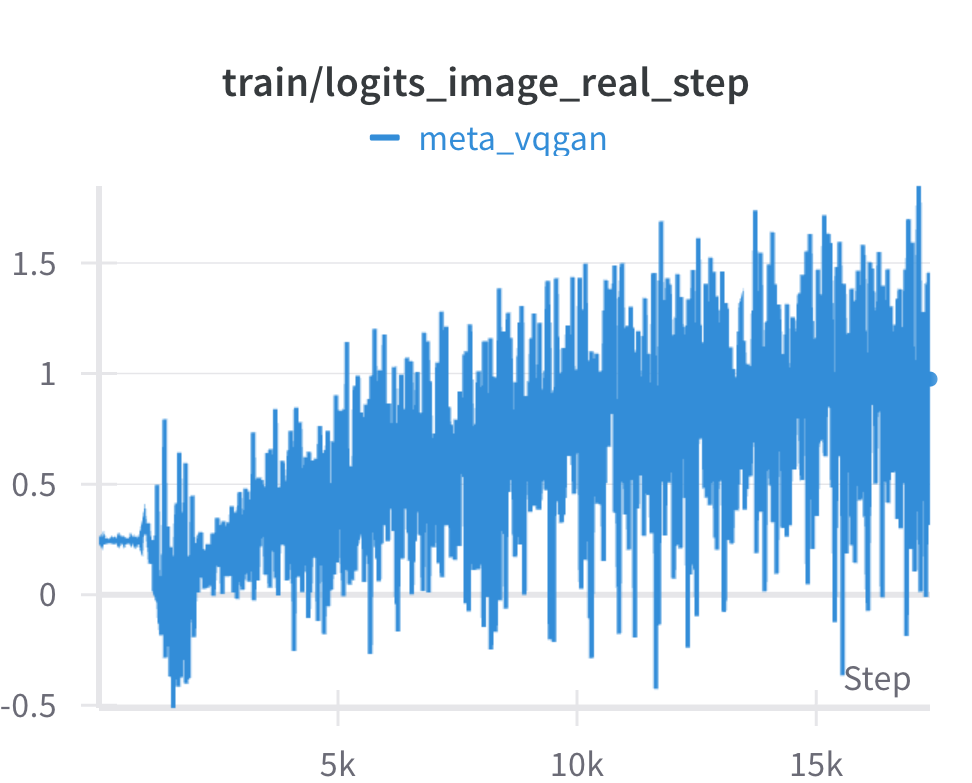
\includegraphics[width=\linewidth]{detailed_engineering/Meta VQGAN/charts/train_logits_image_real_step.png}
%     \caption{Caption}
%     \label{fig:enter-label}
% \end{subfigure}
% \hfill
% \begin{subfigure}[h]{.45\linewidth}
%     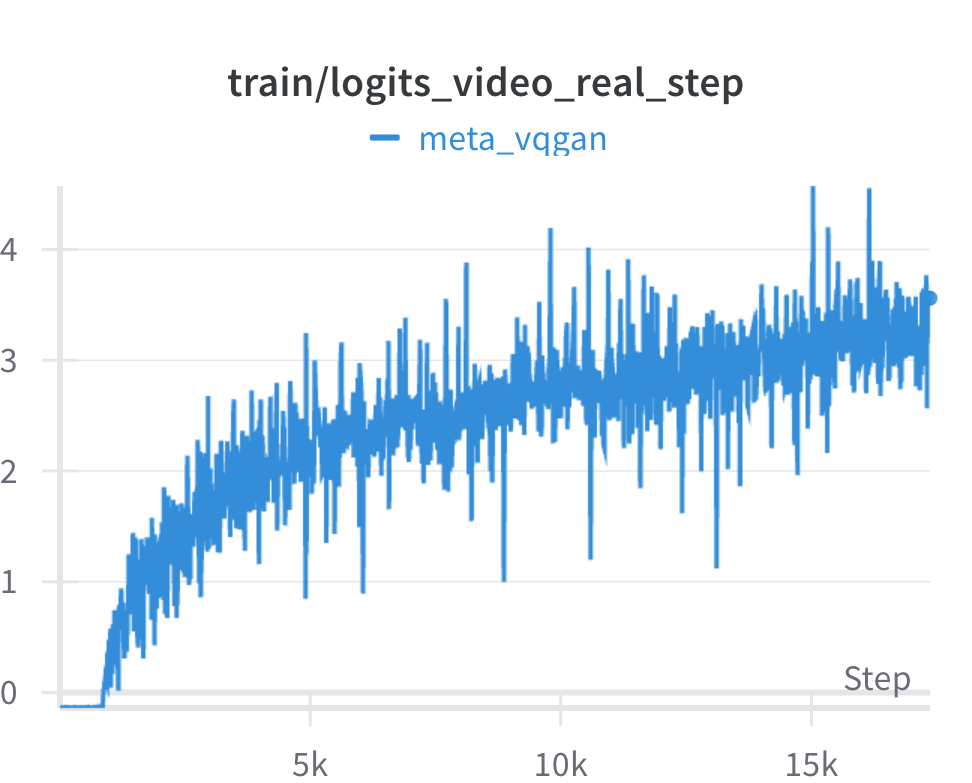
\includegraphics[width=\linewidth]{detailed_engineering/Meta VQGAN/charts/train_logits_video_real_step.png}
%     \caption{Caption}
%     \label{fig:enter-label}
% \end{subfigure}
\hfill
\begin{subfigure}[h]{.45\linewidth}
    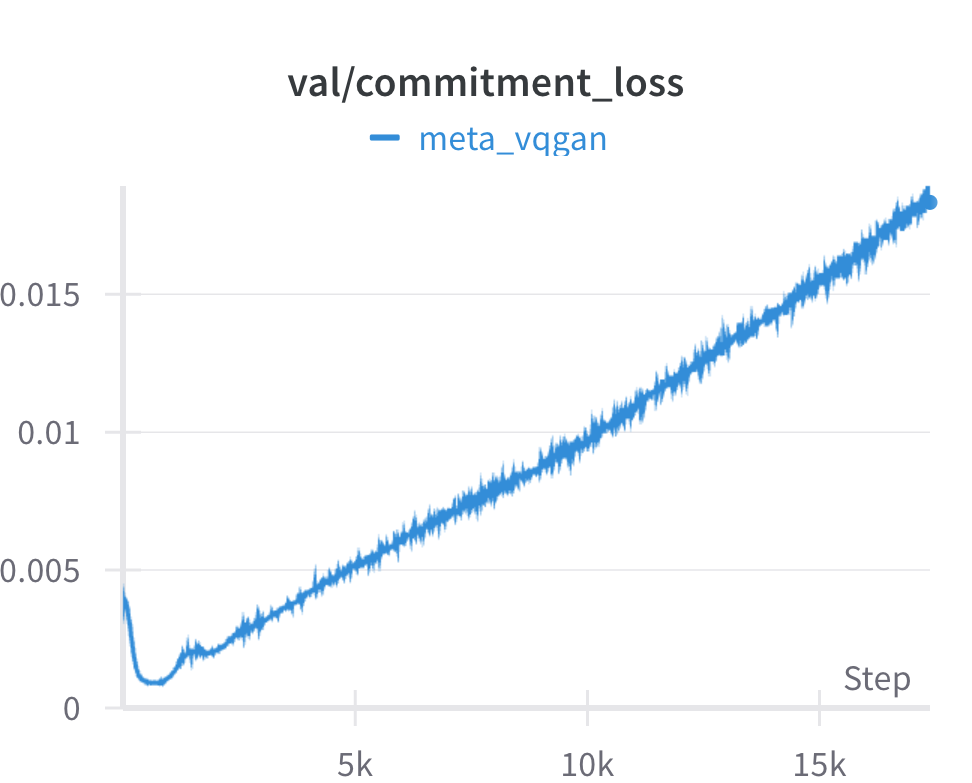
\includegraphics[width=\linewidth]{detailed_engineering/Meta VQGAN/charts/val_commitment_loss.png}
    \caption{Caption}
    \label{fig:enter-label}
\end{subfigure}
\hfill
\begin{subfigure}[h]{.45\linewidth}
    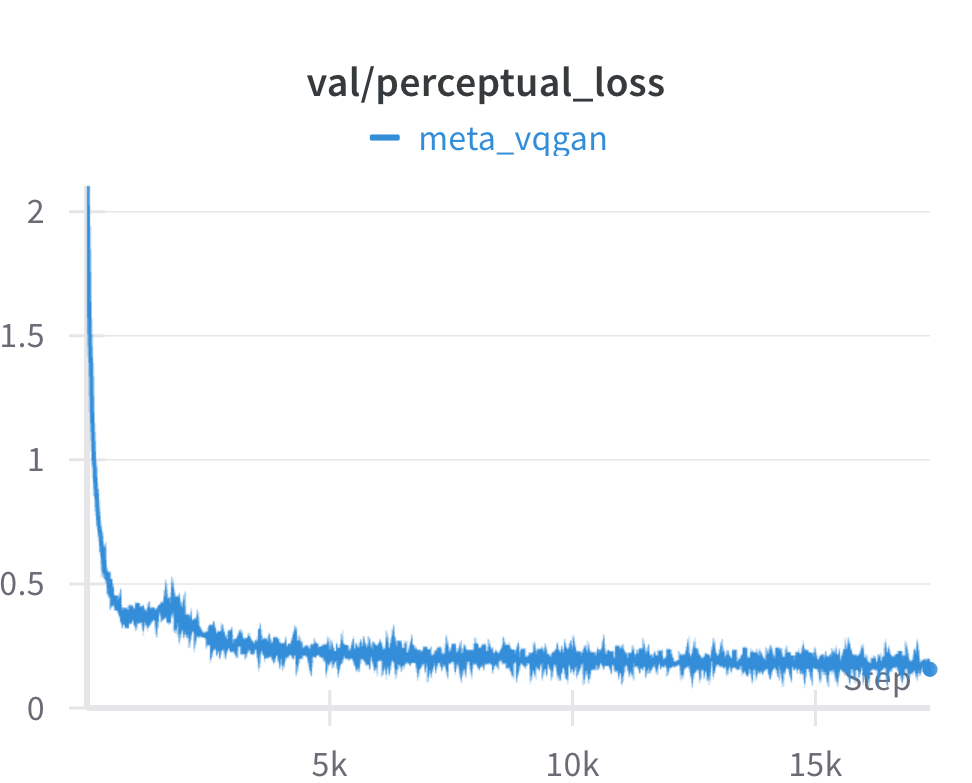
\includegraphics[width=\linewidth]{detailed_engineering/Meta VQGAN/charts/val_perceptual_loss.png}
    \caption{Caption}
    \label{fig:enter-label}
\end{subfigure}
\end{figure}


\paragraph{Results}

\newpage
\paragraph{Medical Diffusion DDPM}
\paragraph{Model configuration}

% \paragraph{Training}
% \begin{figure}[H]
% \centering
% \begin{subfigure}[h]{.45\linewidth}
%     \includegraphics[width=\linewidth]{detailed_engineering/}
%     \caption{Caption}
%     \label{fig:enter-label}
% \end{subfigure}
% \hfill
% \begin{subfigure}[h]{.45\linewidth}
%     \includegraphics[width=\linewidth]{detailed_engineering/Monai Autoencoder/charts/Section-4-Panel-2-bm1y05a9m.png}
%     \caption{Caption}
%     \label{fig:enter-label}
% \end{subfigure}
% \hfill
% \begin{subfigure}[h]{.45\linewidth}
%     \includegraphics[width=\linewidth]{detailed_engineering/Monai Autoencoder/charts/Section-4-Panel-3-dkwhik6ki.png}
%     \caption{Caption}
%     \label{fig:enter-label}
% \end{subfigure}
% \hfill
% \begin{subfigure}[h]{.45\linewidth}
%     \includegraphics[width=\linewidth]{detailed_engineering/Monai Autoencoder/charts/Section-4-Panel-4-d216pe2qa.png}
%     \caption{Caption}
%     \label{fig:enter-label}
% \end{subfigure}
% \hfill
% \begin{subfigure}[h]{.45\linewidth}
%     \includegraphics[width=\linewidth]{detailed_engineering/Monai Autoencoder/charts/Section-4-Panel-5-z2xepgyu7.png}
%     \caption{Caption}
%     \label{fig:enter-label}
% \end{subfigure}
% \end{figure}


\paragraph{Results}
